\chapter{Introduction to clustering, segmentation and connected components}
In this tutorial we'll create an application that demonstrates how an image can be 
broken into a number of regions. The process of separating an image into regions, 
or segments, is called \textbf{segmentation}. Segmentation is a widely studied area in 
computer vision. Researchers often try to optimise their segmentation algorithms 
to try and separate the \textbf{objects} in the image from the \textbf{background}.

To get started, create a new OpenIMAJ project using the Maven archetype, 
import it into your IDE, and delete the sample code from within the generated 
\verb+main()+ method of the \verb+App+ class. In the \verb+main()+ method, 
start by adding code to load an image (choose your own image):
\begin{lstlisting}[language=java]
MBFImage input = ImageUtilities.readMBF(
   new URL("http://..."));
\end{lstlisting}

To segment our image we are going to use a machine 
\marginpar{K-Means initialises cluster centroids with randomly selected data points
and then iteratively assigns the data points to their closest cluster and updates 
the centroids to the mean of the respective clusters data points} 
learning technique called 
\textbf{clustering}. Clustering algorithms automatically group similar things together. In our 
case, we'll use a popular clustering algorithm called \textbf{K-Means} clustering to group 
together all the similar colours in our image. Each group of similar colours is 
known as a \textbf{class}. The K-means clustering algorithm requires you set the number 
of classes you wish to find \textbf{a priori} (i.e. beforehand). 

Colours in our input image are represented in \textbf{RGB colour space}; that is each pixel is 
represented as three numbers corresponding to a red, green and blue value. In order 
to measure the similarity of a pair of colours the ``distance'' between the colours in 
the colour space can be measured. \marginpar{The Euclidean distance is the straight-line 
distance between two points.} Typically, the distance measured is the \textbf{Euclidean} 
distance. Unfortunately, distances in RGB colour space do not reflect what humans perceive as 
similar/dissimilar colours. In order to work-around this problem it is common to transform 
an image into an alternative colour space. The \textbf{Lab colour space} (pronounced as 
separate letters, L A B) is specifically designed so that the Euclidean distance between 
colours closely matches the perceived similarity of a colour pair by a human observer.

\pagebreak
To start our implementation, we'll first apply a colour-space transform to the image:
\begin{lstlisting}[language=java]
input = ColourSpace.convert(input,ColourSpace.CIE_Lab);
\end{lstlisting}
We can then construct the K-Means algorithm:
\begin{lstlisting}[language=java]
FastFloatKMeansCluster cluster = new FastFloatKMeansCluster(3,2,true);
\end{lstlisting}
The first parameter is the dimensionality of the space (3 in this case corresponding 
to the \textbf{L}, \textbf{a}, and \textbf{b} dimensions of the colour vectors). The second 
argument is the number of clusters or classes we wish the algorithm to generate. The final 
boolean flag indicates whether the underlying algorithm should be the ``exact'' K-means algorithm (true) or an 
\textbf{approximate} algorithm (false). The approximate algorithm is much faster than the exact 
algorithm when there is very high-dimensional data; in this case, with only three dimensions, 
the approximate algorithm is not required. The OpenIMAJ K-Means implementation is 
multithreaded and automatically takes advantage of all the processing power it can obtain.

The FastFloatKMeansCluster algorithm takes its input as an array of floating point vectors
(\verb+float[][]+). We can flatten the pixels of an image into the required form using the 
\verb+getPixelVectorNative()+ method:
\begin{lstlisting}[language=java]
float[][] imageData = input.getPixelVectorNative(new float[input.getWidth() * input.getHeight()][3]);
\end{lstlisting}
The K-Means algorithm can then be run to group all the pixels into the requested number of classes:
\begin{lstlisting}[language=java]
cluster.train(imageData);
\end{lstlisting}
Each class or cluster produced by the K-Means algorithm has an index, starting from 0. Each class is 
represented by its centroid (the average location of all the points belonging to the class). We can 
print the coordinates of each centroid:
\begin{lstlisting}[language=java]
float[][] centroids = cluster.getClusters();
for (float[] fs : centroids) {
    System.out.println(Arrays.toString(fs));
}
\end{lstlisting}
Now is a good time to test the code. Running it should print the (\verb+L, a, b+) coordinates of each 
of the classes.

We can now use the \verb+FastFloatKMeansCluster+ to assign each pixel in our image to its respective 
class. This is a process known as \textbf{classification}. The \verb+FastFloatKMeansCluster+ has a method 
called \verb+push_one()+ which takes a vector (the \verb+L, a, b+ value of a single pixel) and 
returns the index of the class that it belongs to. We'll start by creating an image that 
visualises the pixels and their respective classes by replacing each pixel in the input image 
with the centroid of its respective class:
\begin{lstlisting}[language=java]
for (int y=0; y<input.getHeight(); y++) {
    for (int x=0; x<input.getWidth(); x++) {
        float[] pixel = input.getPixelNative(x, y);
        int centroid = cluster.push_one(pixel);
        input.setPixelNative(x, y, centroids[centroid]);
    }
}
\end{lstlisting}
We can then display the resultant image. Note that we need to convert the image back to RGB 
colour space for it to display properly:
\begin{lstlisting}[language=java]
input = ColourSpace.convert(input, ColourSpace.RGB);
DisplayUtilities.display(input);
\end{lstlisting}
Running the code will display an image that looks a little like the original image but with 
as many colours as there are classes. 
\marginpar{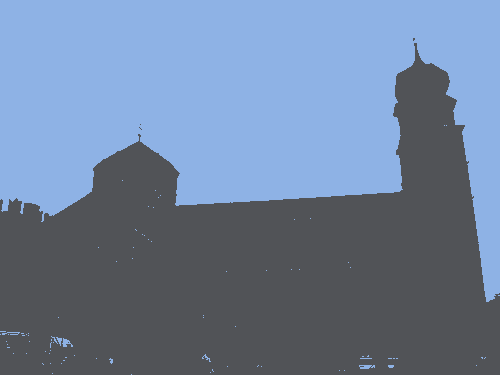
\includegraphics[width=\marginparwidth]{kmeans.png}}

To actually produce a segmentation of the image we need to group together all pixels with 
the same class that are touching each other. Each set of pixels representing a segment is 
often referred to as a \textbf{connected component}. Connected components in OpenIMAJ are
modelled by the \verb+ConnectedComponent+ class.

The \verb+GreyscaleConnectedComponentLabeler+ class can be used to find the connected components:
\begin{lstlisting}[language=java]
GreyscaleConnectedComponentLabeler labeler = new GreyscaleConnectedComponentLabeler();
List<ConnectedComponent> components = labeler.findComponents(input.flatten());
\end{lstlisting}
Note that the \verb+GreyscaleConnectedComponentLabeler+ 
\marginpar{OpenIMAJ also contains a class called \texttt{ConnectedComponent}-\texttt{Labeler} which can
only be used on \textbf{binary} (i.e. pure black and white) \texttt{FImage}s.} 
only processes greyscale images 
(the \verb+FImage+ class) and not the colour image (\verb+MBFImage+ class) that we created. 
The \verb+flatten()+ method on \verb+MBFImage+ merges the colours into grey values by 
averaging their RGB values.

The \verb+ConnectedComponent+ class has many useful methods for extracting information 
about the shape of the region. Lets draw an image with the components numbered on it. We'll use the 
centre of mass of each region to position the number and only render numbers for regions that 
are over a certain size (50 pixels in this case):
\begin{lstlisting}[language=java]
int i = 0;
for (ConnectedComponent comp : components) {
    if (comp.calculateArea() < 50) 
        continue;
    input.drawText("Point:" + (i++), comp.calculateCentroidPixel(), HersheyFont.TIMES_MEDIUM,20);
}
\end{lstlisting}
Finally, we can display the image with the labels:
\begin{lstlisting}[language=java]
DisplayUtilities.display(input);
\end{lstlisting}
\marginpar{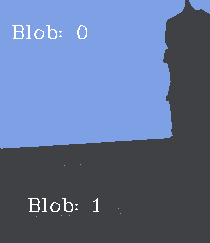
\includegraphics[width=\marginparwidth]{segmented.png}}

\pagebreak
\section*{Exercises}
\subsection*{Exercise 1: The PixelProcessor}
Rather than looping over the image pixels using two for loops, it is possible to use a 
\verb+PixelProcessor+ to accomplish the same task:
\begin{lstlisting}[language=java]
image.processInline(new PixelProcessor<Float[]>() {
    Float[] processPixel(Float[] pixel, Number[]...otherpixels) {
        ...
    }
});
\end{lstlisting}
Can you re-implement the loop that replaces each pixel with its class centroid 
using a \verb+PixelProcessor+? 

What are the advantages and disadvantages of using a \verb+PixelProcessor+?

\subsection*{Exercise 2: A real segmentation algorithm}
The segmentation algorithm we just implemented can work reasonably well, but is rather na\"ive. OpenIMAJ contains an 
implementation of a popular segmentation algorithm called the \verb+FelzenszwalbHuttenlocherSegmenter+. 

Try using the \verb+FelzenszwalbHuttenlocherSegmenter+ for yourself and see how it compares to the 
basic segmentation algorithm we implemented. You can use the \verb+SegmentationUtilities.renderSegments()+ 
static method to draw the connected components produced by the segmenter.

